\documentclass[aspectratio=169, 10pt, xcolor=table]{beamer}

% --- Package Configuration ---
\usepackage{booktabs}   % Table styling
\usepackage{listings}   % Code blocks
\usepackage{tikz}       % Drawing
\usepackage{multimedia} % Video embedding
\usetikzlibrary{shapes, arrows.meta, positioning, fit, backgrounds, shadows, calc}

% --- Theme Settings: FU Berlin Style ---
\usetheme{Madrid}

% 1. Define FU Berlin Official Colors
\definecolor{FUblue}{RGB}{0, 51, 102}    % Dark Blue (Primary)
\definecolor{FUgreen}{RGB}{153, 204, 0}  % Bright Green (Accent)
\definecolor{FUgray}{RGB}{235, 235, 235} % Light Gray for backgrounds

% 2. Apply Structure Colors
\usecolortheme[named=FUblue]{structure} 

% 3. Specific Overrides for FU Look
\setbeamercolor{frametitle}{bg=FUblue, fg=white}        % Header: Blue bg, White text
\setbeamercolor{framesubtitle}{fg=FUgreen}              % Subtitle: FU Green for contrast
\setbeamercolor{title}{bg=FUblue, fg=white}             % Title page header
\setbeamercolor{author}{fg=FUblue}
\setbeamercolor{institute}{fg=black}
\setbeamercolor{date}{fg=gray}

\setbeamercolor{block title}{bg=FUblue, fg=white}
\setbeamercolor{block body}{bg=FUblue!5, fg=black}      % Very light blue tint for blocks

% Table row colors
\rowcolors{2}{FUblue!5}{white}

% --- Custom Colors & Styles ---
\definecolor{codebg}{rgb}{0.95,0.95,0.95}

% Code Block Style
\lstset{
    backgroundcolor=\color{codebg},
    basicstyle=\ttfamily\footnotesize,
    breaklines=true,
    keywordstyle=\color{FUblue}\bfseries, 
    commentstyle=\color{gray}\itshape,
    stringstyle=\color{FUgreen!80!black},
    frame=single,
    showstringspaces=false,
    escapechar=@
}

% TikZ Common Styles (Adapted to FU Colors)
\tikzset{
    basicbox/.style={
        rectangle, 
        rounded corners, 
        draw=FUblue!80, 
        fill=white, 
        very thick, 
        align=center, 
        minimum height=0.8cm,
        drop shadow
    },
    arrow/.style={
        -{Stealth[length=3mm]}, 
        thick,
        color=FUblue
    },
    biarrow/.style={
        arrows={Stealth[length=3mm]-Stealth[length=3mm]}, 
        thick,
        color=FUblue
    },
    % Sequence Diagram Styles
    seqline/.style={
        draw,
        dashed,
        color=gray!80
    },
    seqbox/.style={
        rectangle,
        draw=black,
        fill=white,
        thick,
        font=\scriptsize\bfseries, 
        minimum height=0.5cm,
        minimum width=1.2cm,
        drop shadow,
        align=center
    },
    seqmsg/.style={
        ->,
        >=Stealth,
        thick,
        color=FUblue,
        font=\scriptsize 
    },
    seqret/.style={
        ->,
        >=Stealth,
        thick,
        dashed,
        color=FUblue,
        font=\scriptsize
    },
    % Helper for visibility
    invisible/.style={opacity=0},
    visible on/.style={alt={#1{}{invisible}}},
    alt/.code args={<#1>#2#3}{%
      \alt<#1>{\pgfkeysalso{#2}}{\pgfkeysalso{#3}} % \pgfkeysalso doesn't exist by default like this in all versions, 
      % but beamer provides \alt. A simpler way for nodes is strictly using \onslide logic outside or customized styles.
      % For this code, I will use standard \onslide<x-> logic around draw commands to be safe.
    },
}

% --- Title Information ---
\title[Smart Home Demo Lab Team 2 Update 4 Report]{Smart Home Demo Lab Team 2 Update 4 Report}
\author[Team 2]{Yixue Wang, Linghao Dong, Yang Xiao, Chenxu Liu, Tong Lu}
\date{December 10, 2025}

\begin{document}

% --- Cover ---
\begin{frame}
    \titlepage
\end{frame}

% --- Slide 1: Work Overview ---
\begin{frame}{Overview of Work in the Past Two Weeks}
    \begin{columns}[t]
        \column{0.48\textwidth}
            % First Block appears
            \begin{block}{Application Layer}
                % Items appear 1 by 1
                \begin{itemize}[<+->]
                    \item \textbf{DeviceService}\\
                    Device registration, enable/disable, state sync.
                    \item \textbf{SceneService}\\
                    Scene creation, editing, publishing, disabling.
                    \item \textbf{OrchestrationService}\\
                    Scene execution coordination \& workflow management.
                \end{itemize}
            \end{block}

        \column{0.48\textwidth}
            % Pause before Right Column starts
            \pause
            \begin{block}{Infrastructure Layer}
                \begin{itemize}[<+->]
                    \item \textbf{Data Persistence}\\
                    SQLAlchemy ORM, Repositories.
                    \item \textbf{Event Bus}\\
                    asyncio-based in-memory event pub/sub.
                    \item \textbf{Hardware Communication}\\
                    HTTP Client \& Client Registry.
                    \item \textbf{Logging Module}\\
                    Unified logging configuration.
                \end{itemize}
            \end{block}
    \end{columns}
\end{frame}

% --- Video Slide: Demo ---
\begin{frame}{Demo Video}
    \centering
    \vspace{1em}
    \movie[externalviewer]{
        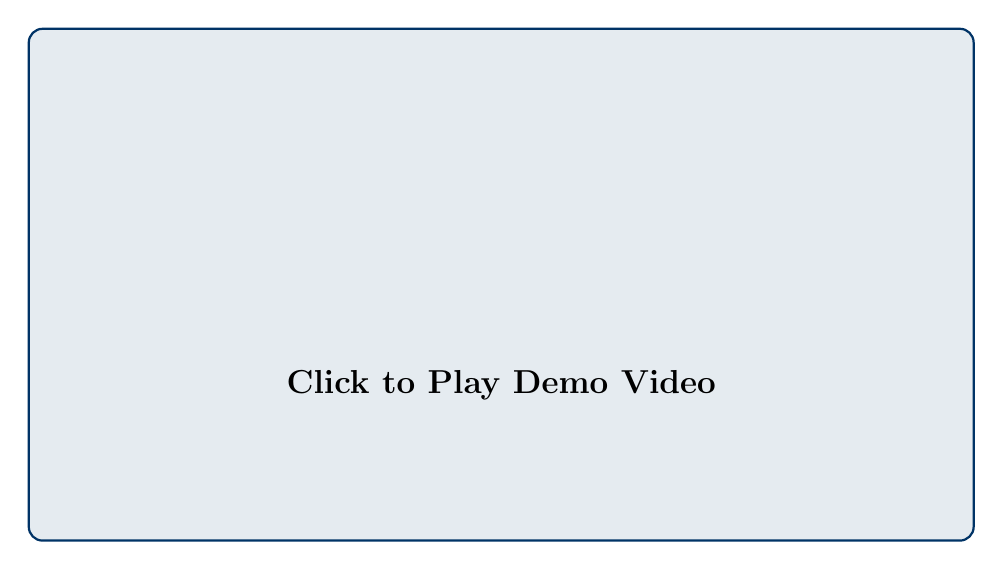
\begin{tikzpicture}
            \node[draw=FUblue, fill=FUblue!10, thick, rounded corners=5pt, minimum width=12cm, minimum height=6.5cm, align=center] {
                \\[1.5cm]
                {\Huge \color{FUblue} $\blacktriangleright$}
                \\[0.5cm]
                {\large \bfseries Click to Play Demo Video}
            };
        \end{tikzpicture}
    }{b892ee2eaf8d0064184b37fc8681f04e_raw.mp4}
\end{frame}

% --- Slide 2: Application Layer - Device Service ---
\begin{frame}{Application Layer - Device Service}
    {\small \color{white} Unified management of smart device lifecycle, providing registration, state sync, and control capabilities.}
    
    \vspace{0.5em}
    % Text appears first
    \onslide<1->{\textbf{Design Concept:} Acts as a mediator, encapsulating device management flows, coordinating domain objects, and publishing events.}
    
    \vspace{1em}
    \begin{columns}
        \column{0.4\textwidth}
            % Wait for key press
            \pause
            \textbf{Dependencies:}
            \vspace{0.5em}
            \resizebox{0.9\textwidth}{!}{
            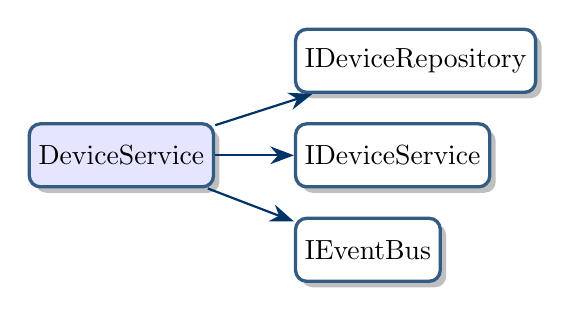
\begin{tikzpicture}[node distance=1cm, transform shape]
                \node[basicbox, fill=blue!10] (svc) {DeviceService};
                \node[basicbox, right=of svc, yshift=1.2cm] (repo) {IDeviceRepository};
                \node[basicbox, right=of svc] (isvc) {IDeviceService};
                \node[basicbox, right=of svc, yshift=-1.2cm] (bus) {IEventBus};
                
                \draw[arrow] (svc) -- (repo);
                \draw[arrow] (svc) -- (isvc);
                \draw[arrow] (svc) -- (bus);
            \end{tikzpicture}
            }
        
        \column{0.6\textwidth}
            % Wait again
            \pause
            \textbf{Functional List}
            \resizebox{\textwidth}{!}{
            \begin{tabular}{l l}
                \toprule
                \textbf{Method} & \textbf{Description} \\
                \midrule
                \texttt{register\_device()} & Register, generate UUID, publish event \\
                \texttt{enable/disable} & Toggle state, publish status change \\
                \texttt{sync\_device\_state()} & Delegate domain service to sync state \\
                \texttt{get\_device(\_by\_id)} & Get device details \\
                \texttt{list\_devices()} & Query list (with filters) \\
                \texttt{delete\_device()} & Delete device \\
                \bottomrule
            \end{tabular}
            }
    \end{columns}
\end{frame}

% --- Slide 3: Application Layer - Scene Service ---
\begin{frame}{Application Layer - Scene Service}
    {\small \color{white} Manages the full lifecycle of scenes and validates scene definitions.}

    \begin{columns}
        \column{0.45\textwidth}
            \onslide<1->{
            \textbf{Scene State Machine}
            \vspace{1em}
            \begin{center}
            \resizebox{0.75\textwidth}{!}{
            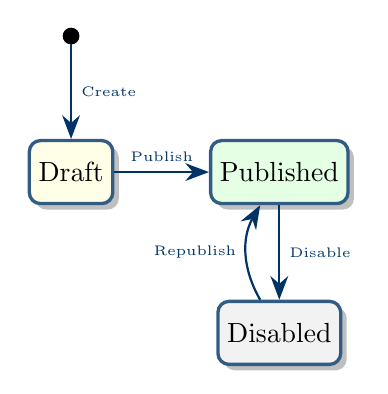
\begin{tikzpicture}[node distance=1.2cm]
                \node[draw, circle, fill=black, inner sep=2pt] (start) {};
                \node[basicbox, below=of start, fill=yellow!10] (draft) {Draft};
                \node[basicbox, right=of draft, fill=green!10] (pub) {Published};
                \node[basicbox, below=of pub, fill=gray!10] (dis) {Disabled};
                
                \draw[arrow] (start) -- node[right, font=\tiny]{Create} (draft);
                \draw[arrow] (draft) -- node[above, font=\tiny]{Publish} (pub);
                \draw[arrow] (pub) -- node[right, font=\tiny]{Disable} (dis);
                \draw[arrow, bend left] (dis) to node[left, font=\tiny]{Republish} (pub);
            \end{tikzpicture}
            }
            \end{center}
            }

        \column{0.55\textwidth}
            \pause
            \textbf{Functional List}
            \resizebox{\textwidth}{!}{
            % Standard table
            \begin{tabular}{l l}
                \toprule
                \textbf{Method} & \textbf{Description} \\
                \midrule
                \texttt{create\_scene()} & Create draft scene \\
                \texttt{update\_scene(\_def)} & Update info/def (w/ validation) \\
                \texttt{publish\_scene()} & Publish (triggers event) \\
                \texttt{disable\_scene()} & Disable (triggers event) \\
                \texttt{get\_scene(\_def)} & Get details/definition \\
                \texttt{list\_scenes} & Query list \\
                \texttt{delete\_scene()} & Delete scene \\
                \bottomrule
            \end{tabular}
            }
    \end{columns}
\end{frame}

% --- Slide 4: Application Layer - Orchestration Service ---
\begin{frame}{Application Layer - Orchestration Service}
    {\small \color{white} Acts as the coordinator of three contexts, triggers execution, and drives the workflow.}

    \vspace{0.2em}
    \begin{columns}[c]
        \column{0.65\textwidth} 
            \textbf{Execution Flow}
            \vspace{0.2em}
            
            \resizebox{\textwidth}{!}{
            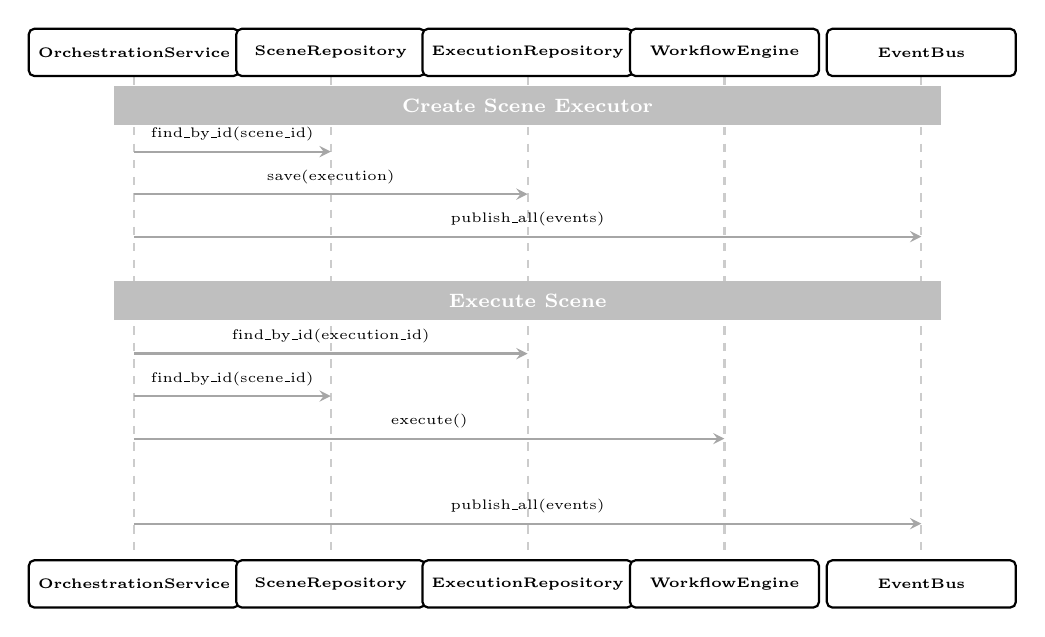
\begin{tikzpicture}[x=2.5cm, y=-0.45cm] 
                
                % --- Simple Clean Styles (matching reference) ---
                \tikzstyle{pbox}=[rectangle, draw=black, fill=white, thick, rounded corners=2pt, font=\tiny\bfseries, minimum width=2.4cm, minimum height=0.6cm, align=center]
                \tikzstyle{msg}=[->, >=stealth, thick, color=gray!70]
                \tikzstyle{lbl}=[font=\tiny, text=black, above, midway] 
                \tikzstyle{phasebar}=[rectangle, fill=gray!50, draw=none, inner sep=4pt, font=\scriptsize\bfseries\color{white}, minimum height=0.5cm, minimum width=10.5cm, align=center]

                % --- Participants (Top) ---
                \node[pbox] (O)  at (0,0) {OrchestrationService};
                \node[pbox] (SR) at (1,0) {SceneRepository};
                \node[pbox] (ER) at (2,0) {ExecutionRepository};
                \node[pbox] (W)  at (3,0) {WorkflowEngine};
                \node[pbox] (EB) at (4,0) {EventBus};

                % --- Lifelines (dashed vertical lines) ---
                \begin{scope}[on background layer]
                    \foreach \x in {O, SR, ER, W, EB} {
                        \draw[dashed, color=gray!40, line width=0.8pt] (\x.south) -- +(0, 14.5);
                    }
                \end{scope}

                % --- PHASE 1: Create Scene Executor ---
                \onslide<1->{
                    \node[phasebar] at (2, 1.5) {Create Scene Executor};
                    \draw[msg] ($(O)+(0,2.8)$) -- node[lbl] {find\_by\_id(scene\_id)} ($(SR)+(0,2.8)$);
                    \draw[msg] ($(O)+(0,4.0)$) -- node[lbl] {save(execution)} ($(ER)+(0,4.0)$);
                    \draw[msg] ($(O)+(0,5.2)$) -- node[lbl] {publish\_all(events)} ($(EB)+(0,5.2)$);
                }
                
                % --- PHASE 2: Execute Scene ---
                \onslide<2->{
                    \node[phasebar] at (2, 7.0) {Execute Scene};
                    \draw[msg] ($(O)+(0,8.5)$)  -- node[lbl] {find\_by\_id(execution\_id)} ($(ER)+(0,8.5)$);
                    \draw[msg] ($(O)+(0,9.7)$)  -- node[lbl] {find\_by\_id(scene\_id)} ($(SR)+(0,9.7)$);
                    \draw[msg] ($(O)+(0,10.9)$) -- node[lbl] {execute()} ($(W)+(0,10.9)$);
                    \draw[msg] ($(O)+(0,13.3)$) -- node[lbl] {publish\_all(events)} ($(EB)+(0,13.3)$);
                }
                
                % --- Bottom Boxes (close lifelines) ---
                \onslide<2->{
                     \node[pbox] at (0,15) {OrchestrationService};
                     \node[pbox] at (1,15) {SceneRepository};
                     \node[pbox] at (2,15) {ExecutionRepository};
                     \node[pbox] at (3,15) {WorkflowEngine};
                     \node[pbox] at (4,15) {EventBus};
                }

            \end{tikzpicture}
            }
        
        \column{0.35\textwidth}
            \onslide<3->{
            \textbf{Functional List}
            \resizebox{\textwidth}{!}{
            \begin{tabular}{l l}
                \toprule
                \textbf{Method} & \textbf{Description} \\
                \midrule
                \texttt{trigger\_execution()} & Triggers execution, creates record \\
                \texttt{execute\_scene()} & Invokes engine to execute scene \\
                \texttt{trigger\_and\_execute()} & Trigger \& execute immediately \\
                \texttt{get\_execution()} & Retrieves execution record \\
                \texttt{get\_execution\_details()} & Gets structured exec details \\
                \texttt{list\_executions()} & Queries execution list \\
                \texttt{list\_executions\_for\_scene()} & Gets all executions for a scene \\
                \bottomrule
            \end{tabular}
            }
            }
    \end{columns}
\end{frame}

% --- Slide 5: Infrastructure Layer - Data Persistence ---
\begin{frame}{Infrastructure Layer - Data Persistence}
    \textbf{Architecture:} Implementation based on SQLAlchemy, supporting SQLite/PostgreSQL.
    
    \vspace{0.5em}
    \begin{columns}[c] 
        \column{0.65\textwidth} 
            \centering
            \resizebox{0.9\textwidth}{!}{
            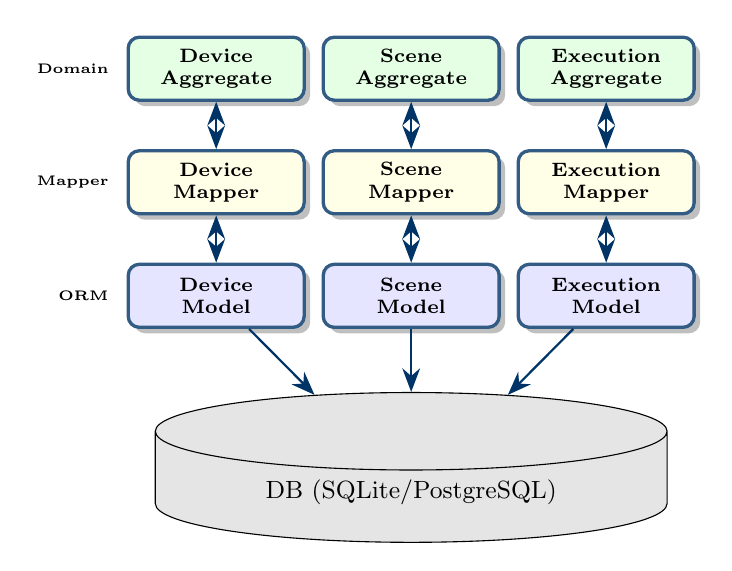
\begin{tikzpicture}[node distance=0.6cm and 0.2cm] 
                \tikzstyle{dombox}=[basicbox, fill=green!10, font=\scriptsize\bfseries, text width=2.0cm]
                \tikzstyle{mapbox}=[basicbox, fill=yellow!10, font=\scriptsize\bfseries, text width=2.0cm]
                \tikzstyle{ormbox}=[basicbox, fill=blue!10, font=\scriptsize\bfseries, text width=2.0cm]

                % --- Layer 1: Domain (Visible on slide 1+) ---
                \onslide<1->{
                    \node[dombox] (sa) {Scene\\Aggregate};
                    \node[dombox, left=of sa] (da) {Device\\Aggregate};
                    \node[dombox, right=of sa] (ea) {Execution\\Aggregate};
                    \node[fit=(da)(sa)(ea), inner sep=0.1cm, label=left:{\tiny\bfseries Domain}] (l1) {};
                }

                % --- Layer 2: Mapper (Visible on slide 2+) ---
                \onslide<2->{
                    \node[mapbox, below=of sa] (sm) {Scene\\Mapper};
                    \node[mapbox, below=of da] (dm) {Device\\Mapper};
                    \node[mapbox, below=of ea] (em) {Execution\\Mapper};
                    \node[fit=(dm)(sm)(em), inner sep=0.1cm, label=left:{\tiny\bfseries Mapper}] (l2) {};
                    \draw[biarrow] (da) -- (dm);
                    \draw[biarrow] (sa) -- (sm); 
                    \draw[biarrow] (ea) -- (em); 
                }

                % --- Layer 3: ORM & DB (Visible on slide 3+) ---
                \onslide<3->{
                    \node[ormbox, below=of sm] (smod) {Scene\\Model};
                    \node[ormbox, below=of dm] (dmod) {Device\\Model};
                    \node[ormbox, below=of em] (emod) {Execution\\Model};
                    \node[fit=(dmod)(smod)(emod), inner sep=0.1cm, label=left:{\tiny\bfseries ORM}] (l3) {};
                    
                    \node[draw, cylinder, shape border rotate=90, aspect=0.25, fill=gray!20, minimum height=0.8cm, minimum width=6.5cm, below=0.8cm of smod, align=center, font=\small] (db) {DB (SQLite/PostgreSQL)};
                    
                    \draw[biarrow] (dm) -- (dmod); \draw[arrow] (dmod) -- (db);
                    \draw[biarrow] (sm) -- (smod); \draw[arrow] (smod) -- (db);
                    \draw[biarrow] (em) -- (emod); \draw[arrow] (emod) -- (db);
                }
            \end{tikzpicture}
            }

        \column{0.35\textwidth}
            % Key features appear after diagram is fully built (Slide 4+)
            \pause \pause \pause 
            \textbf{Key Features}
            \begin{itemize}[<+->]
                \setlength\itemsep{1em}
                \item \textbf{Isolation}: Strict boundaries.
                \item \textbf{Mapping}: Domain $\leftrightarrow$ ORM.
                \item \textbf{Repository}: Encapsulates data access.
            \end{itemize}
    \end{columns}
\end{frame}

% --- Slide 6: Infrastructure Layer - Event Bus ---
\begin{frame}[fragile]{Infrastructure Layer - Event Bus}
    {\small \color{white} Decouples context communication, based on asyncio.PriorityQueue.}

    \begin{columns}
        \column{0.5\textwidth}
            \textbf{Features}
            \vspace{0.5em}
            % List items 1 by 1
            \begin{itemize}[<+->]
                \item \textbf{Priority}: HIGH $>$ NORMAL $>$ LOW
                \item \textbf{Lifecycle}: \texttt{start()} / \texttt{stop()}
                \item \textbf{Handlers}: Sync/Async support
                \item \textbf{Extensibility}: Interface ready for MQ
            \end{itemize}

        \column{0.5\textwidth}
            % Pause before Code block
            \pause
            \textbf{Core Interface Definition}
            \begin{lstlisting}[language=Python]
class IEventBus:
    # Publish single event
    async def publish(event, priority)
    
    # Publish batch
    async def publish_all(events)
    
    # Subscribe to event type
    def subscribe(event_type, handler)
    
    # Unsubscribe
    def unsubscribe(event_type, handler)
            \end{lstlisting}
    \end{columns}
\end{frame}

% --- Slide 7: Infrastructure Layer - Hardware Communication ---
\begin{frame}{Infrastructure Layer - Hardware Communication}
    {\small \color{white} Abstracts platform differences, provides unified control interface.}

    \begin{columns}[t]
        \column{0.55\textwidth}
            \textbf{Layered Design Architecture}
            \vspace{1em}
            \begin{center}
            \resizebox{0.95\textwidth}{!}{ 
            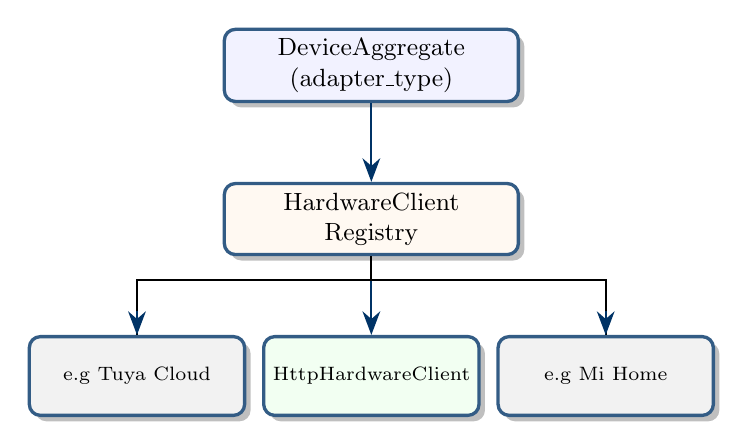
\begin{tikzpicture}[node distance=1cm]
                \tikzstyle{widebox}=[basicbox, font=\small, text width=3.5cm]
                \tikzstyle{clientbox}=[basicbox, font=\scriptsize, text width=2.5cm, minimum height=1cm]

                % Top (Slide 1)
                \onslide<1->{
                    \node[widebox, fill=blue!5] (agg) {DeviceAggregate\\(adapter\_type)};
                }
                
                % Middle (Slide 2)
                \onslide<2->{
                    \node[widebox, fill=orange!5, below=of agg] (reg) {HardwareClient\\Registry};
                    \draw[arrow] (agg) -- (reg);
                }
                
                % Bottom (Slide 3)
                \onslide<3->{
                    \node[clientbox, fill=green!5, below=of reg] (ha) {HttpHardwareClient\\};
                    \node[clientbox, fill=gray!10, left=0.2cm of ha] (tuya) {e.g Tuya Cloud\\};
                    \node[clientbox, fill=gray!10, right=0.2cm of ha] (mi) {e.g Mi Home\\};
                    
                    \draw[arrow] (reg) -- (ha);
                    \draw[thick] (reg.south) -- ++(0,-0.3) -| (tuya.north);
                    \draw[arrow] (tuya.north) ++(0,0.3) -- (tuya.north); 
                    \draw[thick] (reg.south) -- ++(0,-0.3) -| (mi.north);
                    \draw[arrow] (mi.north) ++(0,0.3) -- (mi.north); 
                }
            \end{tikzpicture}
            }
            \end{center}

        \column{0.45\textwidth}
            % Table appears after Diagram (Slide 4)
            \pause \pause \pause
            \textbf{HttpHardwareClient}
            \vspace{1em}
            \begin{tabular}{ll}
                \toprule
                \textbf{Feature} & \textbf{Description} \\
                \midrule
                Platform & API \\
                Auth &  Token \\
                Methods & \texttt{call}, \texttt{get} \\
                \bottomrule
            \end{tabular}
    \end{columns}
\end{frame}

% --- Slide 8: Next Steps ---
\begin{frame}{Next Steps}
    \textbf{Pending Tasks}
    % Table appears first
    \begin{table}
        \rowcolors{2}{gray!10}{white}
        \begin{tabular}{c l l}
            \toprule
            \textbf{\#} & \textbf{Task} & \textbf{Description} \\
            \midrule
            1 & \textbf{Controllers Layer} & REST API, DTO, FastAPI Config \\
            2 & \textbf{Frontend} & UI Development \\
            3 & \textbf{E2E Testing} & Full business flow verification \\
            4 & \textbf{Documentation} & API Docs, Architecture, Guides \\
            \bottomrule
        \end{tabular}
    \end{table}

    \pause
    \vspace{1em}
    \textbf{Future Capabilities}
    % List items 1 by 1
    \begin{itemize}[<+->]
        \item Sub-scene calls (Nested scenes)
        \item Scene version control
        \item Containerization support
    \end{itemize}

    \pause
    \vspace{1em}
    \hrule
    \vspace{0.5em}
    \footnotesize
    \textbf{Team Members}: Yixue Wang, Linghao Dong, Yang Xiao, Chenxu Liu, Tong Lu \\
    Report Date: December 10, 2025
\end{frame}

\end{document}